\documentclass[a4paper,11pt]{report}
\usepackage{fullpage}

\usepackage{"../../info/packages"}
\usepackage{"../../info/nomenclature"}
\usepackage{fullpage}


\title{Material Properties}
\author{Alejandro Campos}

\begin{document}
\maketitle
\tableofcontents

%----------------------------------------------------------------------------------------------------------------------
\chapter{Coulomb scattering}
%----------------------------------------------------------------------------------------------------------------------

%-------------------------------------------------------------------------
\section{Particle equations}
%-------------------------------------------------------------------------
\label{sec:coulomb_particle_equations}
Consider two particles, with positions $\rvec_1=\rvec_1(t)$ and $\rvec_2=\rvec_2(t)$, velocities $\vvec_1=\vvec_1(t)$ and $\vvec_2=\vvec_2(t)$, charges $q_1$ and $q_2$, and masses $m_1$ and $m_2$, respectively. Their positions and velocities are governed by the following equations 
\begin{equation}
    \label{eq:coul_particle_1_pos}
    \frac{d \rvec_1}{dt} = \vvec_1,
\end{equation}
\begin{equation}
    \label{eq:coul_particle_2_pos}
    \frac{d \rvec_2}{dt} = \vvec_2,
\end{equation}
\begin{equation}
    \label{eq:coul_particle_1_vel}
    m_1 \frac{d\vvec_1}{dt} = -\frac{q_1 q_2}{4 \pi \epsilon} \frac{\rvec_2 - \rvec_1}{\left | \rvec_2 - \rvec_1 \right |^3},
\end{equation}
\begin{equation}
    \label{eq:coul_particle_2_vel}
    m_2 \frac{d\vvec_2}{dt} = -\frac{q_1 q_2}{4 \pi \epsilon} \frac{\rvec_1 - \rvec_2}{\left | \rvec_1 - \rvec_2 \right |^3}.
\end{equation}
We note that the above system consists of twelve equations for twelve unknowns. We now introduce the center-of-mass position $\Rvec = \Rvec(t)$, the center-of-mass velocity $\Vvec = \Vvec(t)$, the shifted position $\rvec = \rvec(t)$ and the shifted velocity $\vvec = \vvec(t)$ as follows
\begin{equation*}
    \Rvec = \frac{m_1 \rvec_1 + m_2 \rvec_2}{m_1 + m_2} \qquad \rvec = \rvec_1 - \rvec_2,
\end{equation*}
\begin{equation*}
    \Vvec = \frac{m_1 \vvec_1 + m_2 \vvec_2}{m_1 + m_2} \qquad \vvec = \vvec_1 - \vvec_2
\end{equation*}
Thus, in terms of these new four variables, the particle equations can be written as
\begin{equation}
    \frac{d \Rvec}{dt} = \Vvec,
\end{equation}
\begin{equation}
    \frac{d \Vvec}{dt} = 0 ,
\end{equation}
\begin{equation}
    \label{eq:particle_pos}
    \frac{d \rvec}{dt} = \vvec,
\end{equation}
\begin{equation}
    \label{eq:coul_particle_vel}
    \frac{d \vvec}{dt} = \frac{q_1 q_2}{4\pi \epsilon_0 m_r} \frac{\rvec}{r^3},
\end{equation}
where the reduced mass $m_r$ is given by
\begin{equation}
    \label{eq:coul_reduced_mass}
    \frac{1}{m_r} = \frac{1}{m_1} + \frac{1}{m_2}.
\end{equation}
The first two equations above give the trivial solution $\Vvec = $ constant and $\Rvec$ = $\Rvec(0) + \Vvec t$. Thus, we have reduced the problem from twelve unknowns to six unknowns, namely $\rvec$ and $\vvec$.

%-------------------------------------------------------------------------
\section{Conservation of energy and momentum}
%-------------------------------------------------------------------------
Dotting \cref{eq:coul_particle_vel} by $\vvec$ gives 
\begin{align*}
    \vvec \cdot \frac{d \vvec}{dt} &= \frac{q_1 q_2}{4 \pi \epsilon_0 m_r} \vvec \cdot \frac{\rvec}{r^3} \nonumber \\
    &= \frac{q_1 q_2}{4 \pi \epsilon_0 m_r} \frac{d\rvec}{dt} \cdot \frac{\rvec}{r^3} \nonumber \\
    &= \frac{q_1 q_2}{4 \pi \epsilon_0 m_r} \frac{1}{2} \frac{dr^2}{dt} \frac{1}{r^3} \nonumber \\
    &= \frac{q_1 q_2}{4 \pi \epsilon_0 m_r} \frac{1}{r^2} \frac{dr}{dt} \nonumber \\
    &= -\frac{q_1 q_2}{4 \pi \epsilon_0 m_r} \frac{d}{dt} \left ( \frac{1}{r} \right ).
\end{align*} 
For the left hand side above we have
\begin{equation*}
    \vvec \cdot \frac{d \vvec}{dt} = \frac{1}{2} \frac{d v^2}{dt},
\end{equation*}
and thus we obtain the following expression for conservation of energy
\begin{equation*}
    \frac{d}{dt} \left ( \frac{1}{2} m_r v^2 + \frac{q_1 q_2}{4 \pi \epsilon_0} \frac{1}{r} \right ) = 0.
\end{equation*}

Crossing \cref{eq:coul_particle_vel} by $\rvec$ gives
\begin{equation*}
    \rvec \times \frac{d \vvec}{dt} = \frac{q_1 q_2}{4 \pi \epsilon_0 m_r} \frac{\rvec \times \rvec}{r^3} = 0,
\end{equation*}
and thus
\begin{equation*}
    \frac{d}{dt} \left [ m_r \left ( \rvec \times \vvec \right ) \right ] = 0.
\end{equation*}
That is, angular momentum is conserved. A consequence of this is that the vector $\rvec \times \vvec$ is always pointing in the same direction. Thus, if $\rvec(0)$ and $\vvec(0)$ form a plane, then $\rvec(t)$ and $\vvec(t)$ need to reside within that same plane for all times $t$ so that $\rvec(t) \times \vvec(t)$ points in the same direction as $\rvec(0) \times \vvec(0)$. Therefore, the evolution of the position and velocity are confined to a plane and the problem can be reduced from six unknowns to four unknowns. This planar encounter is depicted in \cref{fig:coulomb_scattering}.
\begin{figure}[ht]
    \centering
    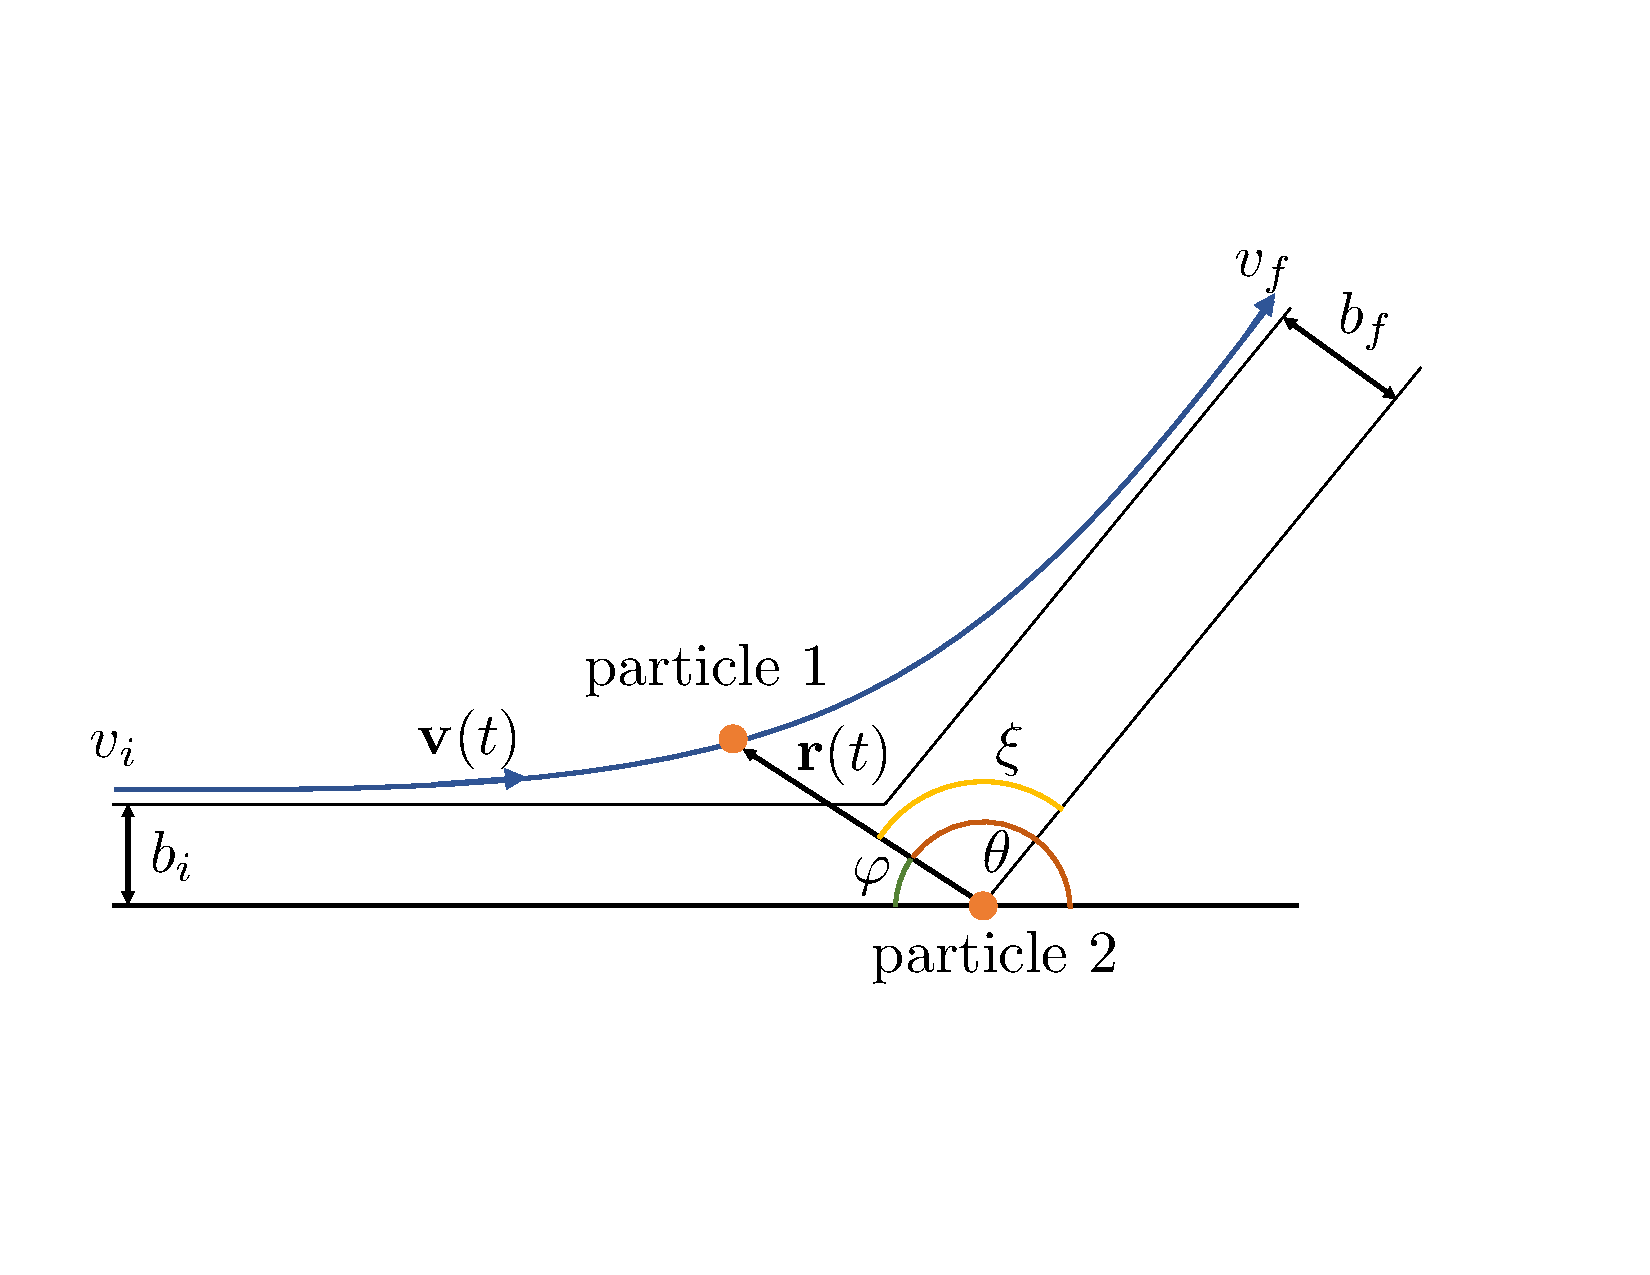
\includegraphics[width=10cm]{../../images/coulomb_scattering.pdf}
    \caption{Depiction of Coulomb scattering.}
    \label{fig:coulomb_scattering}
\end{figure}

If we refer to the plane shown in \cref{fig:coulomb_scattering} as the $x-y$ plane, then one can tell that the angular-momentum vector points in the negative $z$ direction. We will denote the magnitude of the conserved angular momentum by $L$, and thus we can write
\begin{equation}
    \label{eq:coul_cons_angular_momentum}
    m_r \left (\rvec \times \vvec \right ) = -L \hat{\zvec}.
\end{equation}

A consequence of both conservation of energy and momentum is as follows. Consider the two limiting states of particle 1---the initial state $v_i$, $b_i$ and the final state $v_f$, $b_f$. Assuming the potential energy is very low at sufficiently early and late times, conservation of energy gives
\begin{equation}
    \frac{1}{2} m_r v_i^2 = \frac{1}{2} m_r v_f^2,
\end{equation}
that is, $v_i=v_f$ (note that for other scattering processes, e.g.\@ Compton scattering, this is not necessarily the case). For the angular momentum of the initial state we have
\begin{multline}
    \label{eq:coul_cons_angular_momentum_derv1}
    m_r \left ( \rvec_i \times \vvec_i \right ) = m_r \sin(-\theta_i) r_i v_i \hat{\zvec} = - m_r \sin(\theta_i) r_i v_i \hat{\zvec} = - m_r \sin(\pi - \varphi_i) r_i v_i \hat{\zvec} \\
    = - m_r \sin(\varphi_i) r_i v_i \hat{\zvec} = -m_r b_i v_i \hat{\zvec}
\end{multline}
Similarly, for the angular momentum of the final state we have
\begin{equation}
    m_r \left ( \rvec_f \times \vvec_f \right ) = m_r \sin(-\xi_f) r_f v_f  \hat{\zvec} = - m_r \sin(\xi_f) r_f v_f \hat{\zvec} = - m_r b_f v_f \hat{\zvec}.
\end{equation}
Equating the last two relationships gives $m_r b_i v_i = m_r b_f v_f$. Since $v_i = v_f$, we finally have $b_i = b_f = b$. Using \cref{eq:coul_cons_angular_momentum} in \cref{eq:coul_cons_angular_momentum_derv1}, we can also write
\begin{equation}
    \label{eq:coul_cons_angular_momentum_mag}
    L = m_r b v_i.
\end{equation}

%-------------------------------------------------------------------------
\section{Polar coordinates}
%-------------------------------------------------------------------------
\begin{figure}[ht]
    \centering
    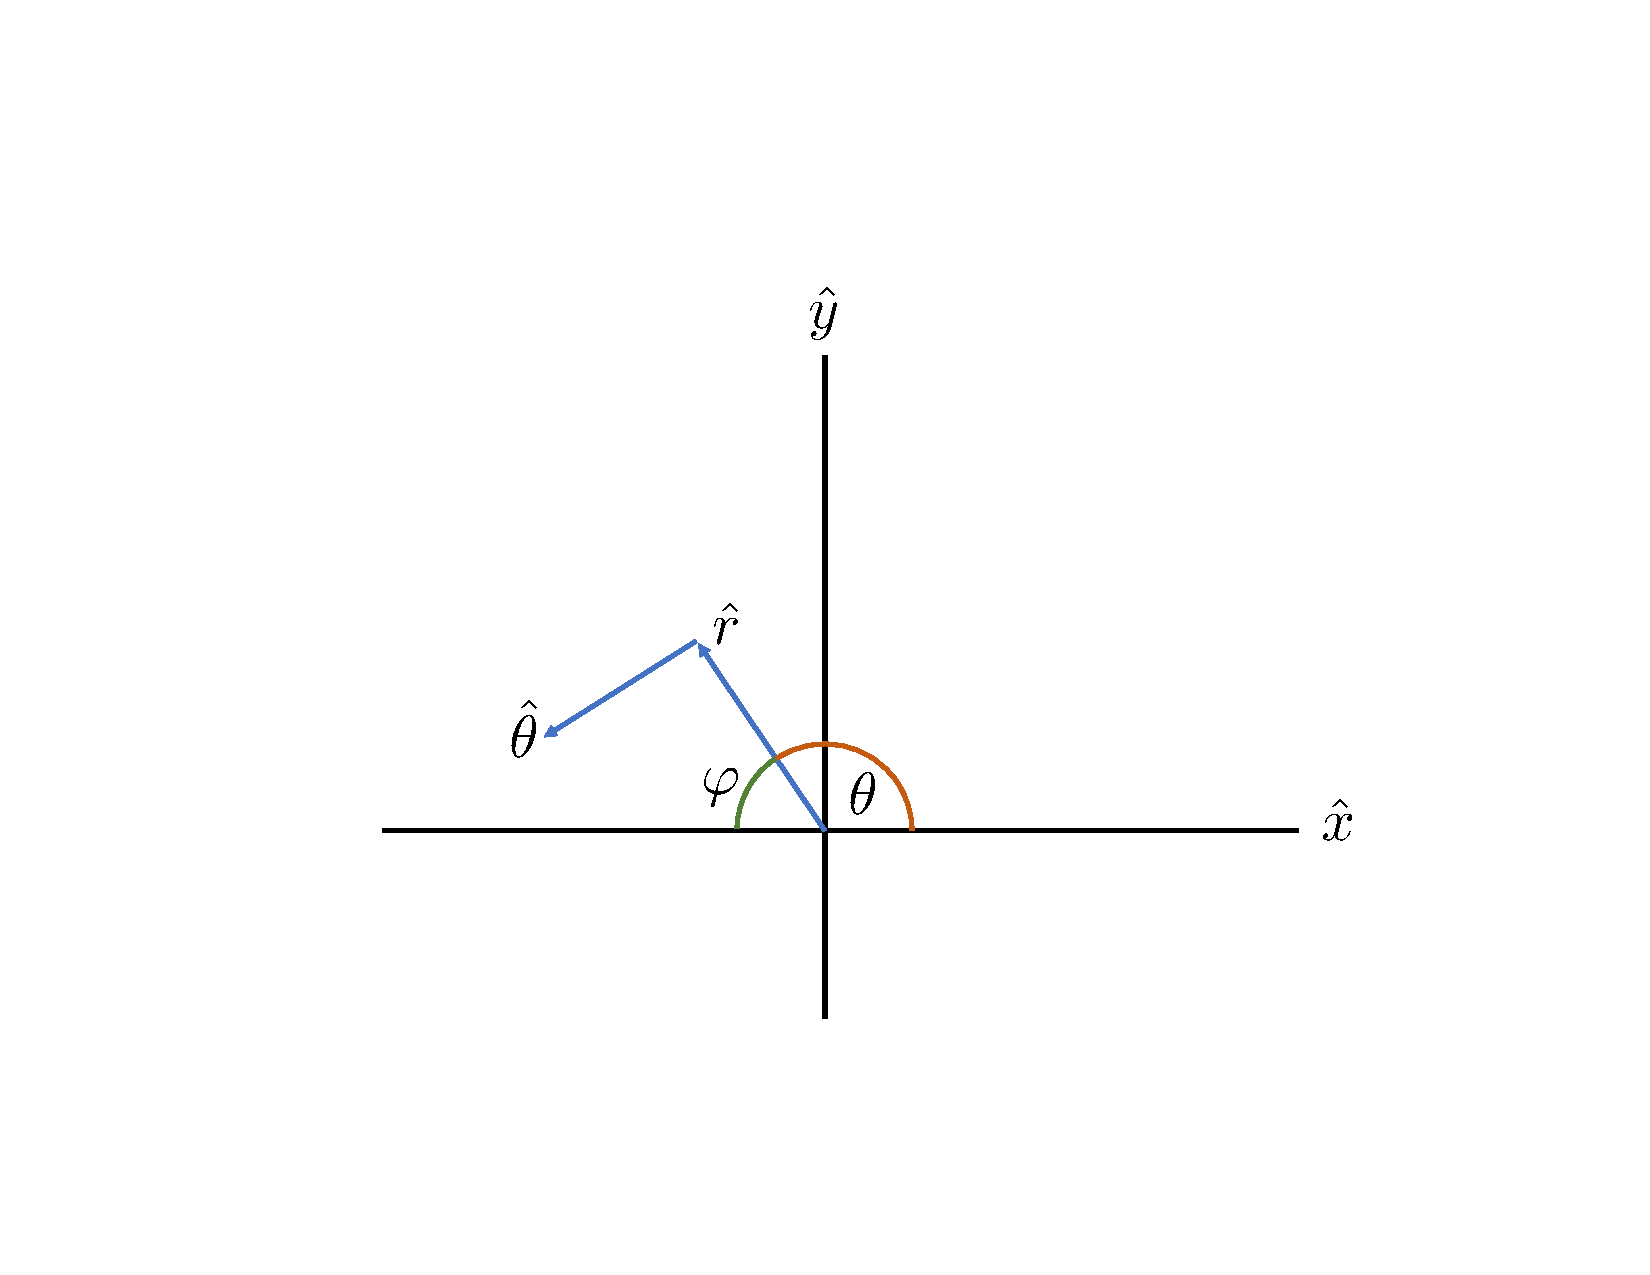
\includegraphics[width=10cm]{../../images/polar_coordinates.pdf}
    \caption{Polar coordinates in plane of interaction.}
    \label{fig:polar_coordinates}
\end{figure}

Using polar coordinates, as shown in \cref{fig:polar_coordinates}, we get
\begin{equation*}
    r_x = r \cos \theta = r \cos ( \pi - \varphi ) = -r \cos \varphi,
\end{equation*}
\begin{equation*}
    r_y = r \sin \theta = r \sin ( \pi - \varphi ) = r \sin \varphi.
\end{equation*}

Also, since $\rvec = r \hat{\rvec}$, we have
\begin{align*}
    \vvec = &\frac{d \rvec}{dt} = \frac{dr}{dt} \hat{\rvec} + r \frac{d\hat{\rvec}}{dt} \nonumber \\
    &= \frac{d r}{dt} \hat{\rvec} + r \frac{d\hat{\rvec}}{d\theta} \frac{d\theta}{dt} \nonumber \\
    &= \frac{dr}{dt} \hat{\rvec} + r \frac{d \theta}{dt} \hat{\bm{\theta}},
\end{align*}
and
\begin{align*}
    \frac{d \vvec}{dt} &= \frac{d^2r}{dt^2} \hat{\rvec} + \frac{dr}{dt} \frac{d\hat{\rvec}}{dt} + \frac{d}{dt} \left ( r \frac{d\theta}{dt} \right ) \hat{\bm{\theta}} + r \frac{d \theta}{dt} \frac{d \hat{\bm{\theta}}}{dt} \nonumber \\
    &= \frac{d^2 r}{dt^2} \hat{\rvec} + \frac{dr}{dt} \frac{d\hat{\rvec}}{d\theta} \frac{d\theta}{dt} + \frac{d}{dt} \left ( r \frac{d\theta}{dt} \right ) \hat{\bm{\theta}} + r \frac{d \theta}{dt} \frac{d \hat{\bm{\theta}}}{d\theta} \frac{d \theta}{dt} \nonumber \\
    &= \frac{d^2r}{dt^2} \hat{\rvec} + \frac{dr}{dt} \frac{d\theta}{dt} \hat{\bm{\theta}} + \frac{d}{dt} \left ( r \frac{d\theta}{dt} \right ) \hat{\bm{\theta}} - r \left ( \frac{d\theta}{dt} \right ) ^2 \hat{\rvec}.
\end{align*}

The radial component of \cref{eq:coul_particle_vel} thus becomes 
\begin{equation*}
    \frac{d^2 r}{dt^2} - r \left ( \frac{d\theta}{dt} \right )^2 = \frac{q_1 q_2}{4 \pi \epsilon_0 m_r} \frac{1}{r^2}.
\end{equation*}
Since $\theta = \pi - \varphi$, we have
\begin{equation}
    \label{eq:coul_particle_position_ode}
    \frac{d^2 r}{dt^2} - r \left ( \frac{d\varphi}{dt} \right )^2 = \frac{q_1 q_2}{4 \pi \epsilon_0 m_r} \frac{1}{r^2}.
\end{equation}

For the angular momentum we have
\begin{equation*}
    m_r \rvec \times \vvec = m_r r \hat{\rvec} \times \left ( \frac{dr}{dt} \hat{\rvec} + r \frac{d\theta}{dt} \hat{\bm{\theta}} \right ) = m_r r^2 \frac{d\theta}{dt} \hat{\zvec}
\end{equation*}
Using \cref{eq:coul_cons_angular_momentum}, we can write the above as
\begin{equation}
    \label{eq:coul_particle_cons_angular_polar}
    m_r r^2 \frac{d\varphi}{dt} = L.
\end{equation}

%-------------------------------------------------------------------------
\section{Particle trajectory}
%-------------------------------------------------------------------------
The goal is to find the radial position of the particle as a function of its angular orientation. That is, we want to find $\tilde{r} = \tilde{r}(\tilde{\varphi})$ such that
\begin{equation}
    \label{eq:coul_particle_position_angle}
    r(t) = \tilde{r}(\varphi(t)).
\end{equation}
To simplify the math, we introduce $\tilde{u} = \tilde{u}(\tilde{\varphi})$ such that $\tilde{u} = 1 / \tilde{r}$. Thus
\begin{equation*}
    \frac{d \tilde{u}}{d\tilde{\varphi}} = -\frac{1}{\tilde{r}^2} \frac{d \tilde{r}}{d\tilde{\varphi}},
\end{equation*}
or, after re-arranging
\begin{equation}
    \label{eq:coul_rgrad_vs_ugrad}
    \frac{d \tilde{r}}{d\tilde{\varphi}} = -\frac{1}{\tilde{u}^2} \frac{d \tilde{u}}{d\tilde{\varphi}}.
\end{equation}

We now proceed as follows. Taking the derivative of $r$, we get
\begin{align}
    \label{eq:coul_particle_derivation_1}
    \frac{dr}{dt} &= \left ( \frac{d \tilde{r}}{d\tilde{\varphi}} \right )_{\tilde{\varphi} = \varphi(t)} \frac{d \varphi}{dt} &&[\cref{eq:coul_particle_position_angle}] \nonumber \\
    &= \left ( -\frac{1}{\tilde{u}^2} \frac{d\tilde{u}}{d\tilde{\varphi}} \right )_{\tilde{\varphi} = \varphi(t)} \frac{d \varphi}{dt} &&[\cref{eq:coul_rgrad_vs_ugrad}]\nonumber \\ 
    &= \left ( -\frac{1}{\tilde{u}^2} \frac{d\tilde{u}}{d\tilde{\varphi}} \right )_{\tilde{\varphi} = \varphi(t)} \frac{L}{m_r r^2} &&[\cref{eq:coul_particle_cons_angular_polar}] \nonumber \\
    &= \left ( -\frac{1}{\tilde{u}^2} \frac{d\tilde{u}}{d\tilde{\varphi}} \frac{L}{m_r \tilde{r}^2} \right )_{\tilde{\varphi} = \varphi(t)} &&[\cref{eq:coul_particle_position_angle}] \nonumber \\
    &= \left ( - \frac{d\tilde{u}}{d\tilde{\varphi}} \frac{L}{m_r} \right )_{\tilde{\varphi} = \varphi(t)}
\end{align}
Taking the derivative of the above, we get
\begin{align}
    \frac{d}{dt} \frac{dr}{dt} &= \left [ \frac{d}{d\tilde{\varphi}} \left ( - \frac{d\tilde{u}}{d\tilde{\varphi}} \frac{L}{m_r} \right ) \right ]_{\tilde{\varphi} = \varphi(t)} \frac{d \varphi}{dt} \nonumber \\
    &= \left ( - \frac{d^2 \tilde{u}}{d\tilde{\varphi}^2} \frac{L}{m_r} \right )_{\tilde{\varphi} = \varphi(t)} \frac{L}{m_r r^2} && [\cref{eq:coul_particle_cons_angular_polar}] \nonumber \\
    &= \left ( - \frac{d^2 \tilde{u}}{d\tilde{\varphi}^2} \frac{L}{m_r} \frac{L}{m_r \tilde{r}^2} \right )_{\tilde{\varphi} = \varphi(t)} && [\cref{eq:coul_particle_position_angle}] \nonumber \\
    &= \left ( - \frac{d^2 \tilde{u}}{d\tilde{\varphi}^2} \frac{L^2 \tilde{u}^2}{m_r^2} \right )_{\tilde{\varphi} = \varphi(t)}
\end{align}
Plugging the last relation into \cref{eq:coul_particle_position_ode} gives
\begin{equation*}
    \left [ - \frac{d^2 \tilde{u}}{d\tilde{\varphi}^2} \frac{L^2 \tilde{u}^2}{m_r^2} - \frac{1}{\tilde{u}} \left ( \frac{L \tilde{u}^2}{m_r} \right )^2 \right ]_{\tilde{\varphi} = \varphi(t)} = \left ( \frac{q_1 q_2}{4 \pi \epsilon_0 m_r} \tilde{u}^2 \right )_{\tilde{\varphi} = \varphi(t)},
\end{equation*}
which, upon re-arranging and dropping the $\varphi(t)$ dependance, becomes
\begin{equation}
    \frac{d^2 \tilde{u}}{d \tilde{\varphi}^2} + \tilde{u} = -\frac{q_1 q_2 m_r}{4 \pi \epsilon_0 L^2}
\end{equation}

Using \cref{eq:coul_cons_angular_momentum_mag} we write the evolution equation for $\tilde{u}$ as
\begin{equation}
    \frac{d^2 \tilde{u}}{d \tilde{\varphi}^2} + \tilde{u} = -\frac{q_1 q_2}{4 \pi \epsilon_0 m_r b^2 v_i^2}.
\end{equation}
Introducing the notation
\begin{equation}
    \label{eq:coul_b90}
    b_{90} = \frac{q_1 q_2}{4 \pi \epsilon_0 m_r v_i^2},
\end{equation}
the evolution equation for $\tilde{u}$ can be simply expressed as
\begin{equation}
    \label{eq:coul_particle_u_equation}
    \frac{d^2 \tilde{u}}{d \tilde{\varphi}^2} + \tilde{u} = -\frac{b_{90}}{b^2}.
\end{equation}

The boundary conditions for \cref{eq:coul_particle_u_equation} are as follows
\begin{equation}
    \label{eq:coul_particle_bc_1}
    \text{as } \varphi(t) \to 0, \quad r(t) \to \infty
\end{equation}
\begin{equation}
    \label{eq:coul_particle_bc_2}
    \text{as } \varphi(t) \to 0, \quad \frac{dr(t)}{dt} \to -v_i
\end{equation}
Given \cref{eq:coul_particle_position_angle}, \cref{eq:coul_particle_bc_1} can only be satisfied if as $\tilde{\varphi} \to 0$, $\tilde{r} \to \infty$. Thus, we also have, as $\tilde{\varphi} \to 0$, $\tilde{u} \to 0$. Similarly, given \cref{eq:coul_particle_derivation_1}, \cref{eq:coul_particle_bc_2} can only be satisfied if as $\tilde{\varphi} \to 0$
\begin{equation*}
    \frac{d\tilde{u}}{d\tilde{\varphi}} \frac{L}{m_r} \to v_i.
\end{equation*}
Using \cref{eq:coul_cons_angular_momentum_mag} we rewrite the above as 
\begin{equation*}
    \frac{d\tilde{u}}{d\tilde{\varphi}} \to \frac{1}{b}.
\end{equation*}

The general solution to \cref{eq:coul_particle_u_equation} is 
\begin{equation*}
    \tilde{u} = A \cos \tilde{\varphi} + B \sin \tilde{\varphi} - \frac{b_{90}}{b^2}.
\end{equation*}
Applying the boundary conditions, we get
\begin{equation*}
    \tilde{u} = \frac{b_{90}}{b^2} \cos \tilde{\varphi} + \frac{1}{b} \sin \tilde{\varphi} - \frac{b_{90}}{b^2},
\end{equation*}
which we finally re-write as
\begin{equation}
    \label{eq:coul_trajectory_eq}
    \frac{1}{\tilde{r}} = \frac{1}{b} \sin \tilde{\varphi} + \frac{b_{90}}{b^2} \left ( \cos \tilde{\varphi} - 1 \right ).
\end{equation}

%-------------------------------------------------------------------------
\section{The scattering angle}
%-------------------------------------------------------------------------
We now drop the tilde notation for the sake of simplicity. That is, for the radial location of an incident particle, we have
\begin{equation}
    \label{eq:coul_trajectory_eq2}
    \frac{1}{r} = \frac{1}{b} \sin \varphi + \frac{b_{90}}{b^2} \left ( \cos \varphi - 1 \right ),
\end{equation}
where $\varphi$ is the independent variable and $r = r(\varphi)$. We want to know the value of $\varphi$ as $r$ goes to infinity. Using \cref{eq:coul_trajectory_eq2}, and labeling this angle as $\varphi_s$, we have
\begin{equation*}
    0 = \sin \varphi_s + \frac{b_{90}}{b} \left ( \cos \varphi_s - 1 \right ).
\end{equation*}
We express the above in terms of the scattering angle $\theta_s = \pi - \varphi_s$,
\begin{equation*}
    0 = \sin (\pi - \theta_s) + \frac{b_{90}}{b} \left [ \cos \left (\pi - \theta_s \right ) - 1 \right ].
\end{equation*}
or
\begin{equation*}
    0 = \sin \theta_s + \frac{b_{90}}{b} \left ( -\cos \theta_s - 1 \right ).
\end{equation*}
Re-writing the above as
\begin{equation*}
    \frac{\cos \theta_s + 1}{\sin \theta_s} = \frac{b}{b_{90}},
\end{equation*}
and using the trig identity $\cot (\theta/2) = (\cos \theta + 1) / \sin \theta$, we get 
\begin{equation}
    \label{eq:coul_scattering_angle}
    \cot \left ( \frac{ \theta_s }{2} \right ) = \frac{b}{b_{90}}.
\end{equation}

%-------------------------------------------------------------------------
\section{The differential cross section}
%-------------------------------------------------------------------------

The differential cross section for Coulomb scattering can be computed by making use of a formula derived in my introductory notes, namely
\begin{equation}
    \label{eq:cross_diff_impact_axi}
    \frac{d\sigma_\theta}{d\Omega} = \frac{b}{\sin \theta_s} \left | \frac{db}{d\theta_s} \right |.
\end{equation}
From \cref{eq:coul_scattering_angle} we get,
\begin{equation}
    \frac{db}{d\theta} = -\frac{b_{90}}{2} \frac{1}{\sin^2 (\theta_s / 2)},
\end{equation}
which, plugging in \cref{eq:cross_diff_impact_axi}, gives
\begin{equation*}
    \frac{d\sigma_\theta}{d\Omega} = \left [ b_{90}\frac{\cot(\theta_s/2)}{\sin \theta_s} \right ] \left [ \frac{b_{90}}{2} \frac{1}{\sin^2 (\theta_s / 2)} \right ].
\end{equation*}
Using the trig identities $\cot(\theta) = \cos(\theta) / \sin(\theta)$ and $\sin(\theta) = 2 \sin(\theta/2) \cos(\theta/2)$ we get
\begin{equation}
    \frac{d\sigma_\theta}{d\Omega} = \frac{b_{90}^2}{4} \frac{1}{\sin^4 (\theta_s/2)}.
\end{equation}

%-------------------------------------------------------------------------
\section{Collision integral}
%-------------------------------------------------------------------------
\begin{equation}
    \Omega_{\alpha \beta}^{(lk)} = \sqrt{ \frac{k_B T}{2 \pi M_{\alpha \beta}} } \int_0^\infty e^{-g^2} g^{2k+3} \phi_{\alpha \beta}^{(l)} \, dg.
\end{equation}
In the above $M_{\alpha \beta}$ is the reduced mass, given by
\begin{equation}
    M_{\alpha \beta} = \frac{M_\alpha M_\beta}{M_\alpha + M_\beta},
\end{equation}
and $\phi^{(l)}_{\alpha \beta}$ is the collision cross section for a given velocity, and is computed as
\begin{equation}
    \phi_{\alpha \beta}^{(l)} = 2 \pi \int_0^\infty \left ( 1 - \cos^l \chi_{\alpha \beta} \right ) b \, db.
\end{equation}
The scattering angle $\chi_{\alpha \beta}$ is given by
\begin{equation}
    \chi_{\alpha \beta} = \pi - 2 \int_{r_{\alpha \beta}^{\text{min}}}^\infty \frac{b}{r^2 \left [ 1 - \frac{b^2}{r^2} - \frac{V_{\alpha \beta (r)}}{g^2 k_B T} \right ]^{1/2} } \, dr.
\end{equation}

For a Coulombic interaction between ions, we can define the natural scale fore the cross-sectional area as
\begin{equation}
    \phi^{(0)}_{\alpha \beta} = \frac{ \pi \left (Z_\alpha Z_\beta e^2 \right)^2}{ \left(2 k_B T\right)^2}.
\end{equation}
Given this definition, we express the collision integral as
\begin{equation}
    \Omega_{\alpha \beta} = \sqrt{ \frac{\pi }{M_{\alpha \beta}}} \frac{( Z_\alpha Z_\beta e^2)^2 }{(2 k_B T )^{3/2}} \mathcal{F}^{lk}_{\alpha \beta},
\end{equation}
where
\begin{equation}
    \mathcal{F}^{(lk)}_{\alpha \beta} = \frac{1}{2 \phi_0} \int_0^\infty e^{-g^2} g^{2k+3} \phi_{\alpha \beta}^{(l)} \, dg
\end{equation}
We note that $\mathcal{F}^{(lk)}_{\alpha \beta} = 4 \mathcal{K}_{lk}(g_{\alpha \beta})$, where $\mathcal{K}_{lk}(g_{\alpha \beta})$ is the notation from the Stanton-Murillo paper.

%----------------------------------------------------------------------------------------------------------------------
\chapter{Transport coefficients}
%----------------------------------------------------------------------------------------------------------------------

%----------------------------------------------------------------------------------------------------------------------
\chapter{Coupling coefficients}
%----------------------------------------------------------------------------------------------------------------------

%-------------------------------------------------------------------------
\section{Momentum exchange collision frequency $\nu_{ei}$}
%-------------------------------------------------------------------------

%-------------------------------------------------------------------------
\section{Electron-ion thermal coupling $w_{ei}$}
%-------------------------------------------------------------------------

\end{document}